\section{Internal coordinates of \texorpdfstring{\cyc}{c-c3h3+} }
\subsection{fc-CCSD(T)/ANO0}
\begin{verbatim}

X
X 1 rd
C 2 r1 1 a90
C 2 r1 1 a90 3 d120
C 2 r1 1 a90 4 d120
H 2 r2 1 a90 3 d0
H 2 r2 1 a90 4 d0
H 2 r2 1 a90 5 d0

rd   =        1.000000613972272
r1   =        0.795954871089489
a90  =       90.000000000000000
d120 =      120.000000000000043
r2   =        1.882733950537102
d0   =        0.000000000000000
\end{verbatim}
    
\subsection{fc-CCSD(T)/ANO1}
\begin{verbatim}
X
X 1 rd
C 2 r1 1 a90
C 2 r1 1 a90 3 d120
C 2 r1 1 a90 4 d120
H 2 r2 1 a90 3 d0
H 2 r2 1 a90 4 d0
H 2 r2 1 a90 5 d0

rd   =        1.000000409314806
r1   =        0.789085470855492
a90  =       90.000000000000000
d120 =      120.000000000000014
r2   =        1.869030138645467
d0   =        0.000000000000000
\end{verbatim}

\subsection{fc-CCSD(T)/ANO2}

\begin{verbatim}
X
X 1 rd
C 2 r1 1 a90
C 2 r1 1 a90 3 d120
C 2 r1 1 a90 4 d120
H 2 r2 1 a90 3 d0
H 2 r2 1 a90 4 d0
H 2 r2 1 a90 5 d0

rd   =        1.000000613972272
r1   =        0.787249651644386
a90  =       90.000000000000000
d120 =      119.999999999999986
r2   =        1.866721530420376
d0   =        0.000000000000000
\end{verbatim}

\section{Internal coordinates of \texorpdfstring{\lin}{l-c3h3+} }

\subsection{fc-CCSD(T)/ANO0}
\begin{verbatim}
H
C 1 r1
X 2 rd 1 a90
C 2 r2 3 a90 1 d180
X 4 rd 2 a90 3 d0
C 4 r3 5 a90 2 d180
H 6 r4 4 a1 5 d0
H 6 r4 4 a1 5 d180

r1   =        1.081884877618416
rd   =        1.000000409314806
a90  =       90.000000000000000
r2   =        1.246343011416748
d180 =      180.000000000000000
d0   =        0.000000000000000
r3   =        1.361798271600899
r4   =        1.094590581296569
a1   =      120.284642603942274
\end{verbatim}

\subsection{fc-CCSD(T)/ANO1}
\begin{verbatim}
H
C 1 r1
X 2 rd 1 a90
C 2 r2 3 a90 1 d180
X 4 rd 2 a90 3 d0
C 4 r3 5 a90 2 d180
H 6 r4 4 a1* 5 d0
H 6 r4 4 a1* 5 d180

r1   =        1.074705266639338
rd   =        1.000000204657382
a90  =       90.000000000000000
r2   =        1.234261558515133
d180 =      180.000000000000000
d0   =        0.000000000000000
r3   =        1.351397370372584
r4   =        1.088292080166718
a1   =      120.373581553220575    
\end{verbatim}


\subsection{fc-CCSD(T)/ANO2}
\begin{verbatim}
H
C 1 r1
X 2 rd 1 a90
C 2 r2 3 a90 1 d180
X 4 rd 2 a90 3 d0
C 4 r3 5 a90 2 d180
H 6 r4 4 a1* 5 d0
H 6 r4 4 a1* 5 d180

r1   =        1.074153711426225
rd   =        1.000000409314806
a90  =       90.000000000000000
r2   =        1.231322876212024
d180 =      180.000000000000000
d0   =        0.000000000000000
r3   =        1.349557181907095
r4   =        1.087405908293182
a1   =      120.356533501538024
\end{verbatim}

\begin{table}[ht]
  % \caption{Vibrational wavenumbers of \cyc calculated in the present study (in \wn ). }
  \caption{Vibrational wavenumbers and IR intensities of \cyc (cm$^{-1}$ and km/mol, respectively).}
    \begin{center}
    \begin{tabular}{rrrrrr} \hline
    
%        \toprule\\ 
        Mode & Harm.$^a$ & Anharm.$^a$ & Harm.$^b$ & Anharm.$^c$ & Int.$^a$ \\ \hline
%        & (this work)&(this work)$^a$&\citeauthor{Botschwina2011}$^b$&\citeauthor{Botschwina2011}$^b$& \citeauthor{HTL2011}$^c$\\
 %       \midrule\\
        $\nu_{1}(a^{'}_1)$   & 3325 & 3194 & 3310 & 3179 & 0 \\ %                   &    & 3182 [0]  & -    \\
        $\nu_{2}(a^{'}_1)$   & 1629 & 1596 & 1642 & 1610 & 0 \\ %                  &    & 1612 [0]  & -    \\
        $\nu_{3}(a^{'}_2)$   & 1028 & 1004 & 1048 & 1024 & 0 \\ %                  &    & 1028 [0]  & -    \\
        $\nu_{4}(e^{'})$     & 3276 & 3142 & 3260 & 3127 & 189 \\ %    3133(1)$^{b}$  & 14 & 3128 [98] & 3182 \\
        $\nu_{5}(e^{'})$     & 1301 & 1266 & 1318 & 1284 & 88 \\ %    1293(1)        & 25 & 1286 [44] & 1293 \\
        $\nu_{6}(e^{'})$     &  940 & 920  &  944 &  925 & 60 \\ %     927(1)         & 19 & 926 [30]  & nc   \\
        $\nu_{7}(a^{''}_2)$  &  763 & 754  &  764 &  754 & 69 \\ %     757(1)         & 20 & 756 [72]  & nc   \\
        $\nu_{8}(e^{''})$    & 1007 & 989  & 1017 & 1000 & 0 \\ %                  &    & 1002 [0]  & -    \\
                \bottomrule
        \hline
    \end{tabular}
    \end{center}
    $^a$ fc-CCSD(T)/ANO0. IR intensity obtained via VPT2. \\
    $^b$ fc-CCSD(T)/ANO2\\
    $^c$ From fc-CCSD(T)/ANO2 harmonic wavenumbers and fc-CCSD(T)/ANO0 anharmonic corrections.
\end{table}

\begin{table}[ht]
  \caption{Vibrational wavenumbers and IR intensities of \cycD (cm$^{-1}$ and km/mol, respectively); CCSD(T)/ANO1 anharmonic force field.}
    \begin{center}
    \begin{tabular}{rrrrrr} \hline
    
%        \toprule\\ 
        Mode & Harm.$^a$ & Anharm.$^a$ & Harm.$^b$ & Anharm.$^c$ & Int.$^a$ \\ \hline
%        & (this work)&(this work)$^a$&\citeauthor{Botschwina2011}$^b$&\citeauthor{Botschwina2011}$^b$& \citeauthor{HTL2011}$^c$\\
 %       \midrule\\
        $\nu_{1}(a^{'}_1)$ & 2552 & 2475 & 2552 & 2474 & 0  \\ % sym. CD str.              &         &    & 2474 [0]    \\
        $\nu_{2}(a^{'}_1)$ & 1501 & 1472 & 1507 & 1478 & 0  \\ % sym. CCC str.             &         &    & 1478 [0]    \\
        $\nu_{3}(a^{'}_2)$ &  845 &  831 &  852 &  838 & 0  \\ % in-plane internal torsion &         &    & 838  [0]   \\
        $\nu_{4}(e^{'})$   & 2420 & 2341 & 2419 & 2340 & 64  \\ %asym. CD str              & 2343(1) & 30 & 2340 [32]  \\ 
        $\nu_{5}(e^{'})$   & 1266 & 1236 & 1273 & 1244 & 66  \\ % asym. CCC ring str.       & 1249(1) & 25 & 1244 [33]  \\
        $\nu_{6}(e^{'})$   &  684 &  673 &  684 &  673 & 28  \\ % in-plane CD scissoring    & 674(1)  & 19 & 673  [14]  \\
        $\nu_{7}(a^{''}_2)$&  561 &  556 &  561 &  556 & 29  \\ % sym. CD bending \oplus    & 556(1)  & 15 & 556  [29]  \\
        $\nu_{8}(e^{''})$  &  823 &  813 &  827 &  817 & 0  \\ % asym. CD bending \oplus   &         &    & 817  [0]   \\
                \bottomrule
        \hline
    \end{tabular}
    \end{center}
    $^a$ fc-CCSD(T)/ANO1. IR intensity obtained via VPT2.\\
    $^b$ fc-CCSD(T)/ANO2\\
    $^c$ From fc-CCSD(T)/ANO2 harmonic wavenumbers and fc-CCSD(T)/ANO1 anharmonic corrections.
\end{table}

\begin{table}[ht]
  % \caption{Vibrational wavenumbers of BLA calculated in the present study (in \wn ). }
  \caption{Vibrational wavenumbers and IR intensities of \cycD (cm$^{-1}$ and km/mol, respectively); CCSD(T)/ANO0 anharmonic force field.}
    \begin{center}
    \begin{tabular}{rrrrrr} \hline
    
%        \toprule\\ 
        Mode & Harm.$^a$ & Anharm.$^a$ & Harm.$^b$ & Anharm.$^c$ & Int.$^a$\\ \hline
%        & (this work)&(this work)$^a$&\citeauthor{Botschwina2011}$^b$&\citeauthor{Botschwina2011}$^b$& \citeauthor{HTL2011}$^c$\\
 %       \midrule\\
        $\nu_{1}(a^{'}_1)$ & 2560 & 2481 & 2552 & 2473 & 0  \\ % sym. CD str.              &         &    & 2474 [0]    \\
        $\nu_{2}(a^{'}_1)$ & 1497 & 1466 & 1507 & 1477 & 0  \\ % sym. CCC str.             &         &    & 1478 [0]    \\
        $\nu_{3}(a^{'}_2)$ &  835 &  818 &  852 &  835 & 0  \\ % in-plane internal torsion &         &    & 838  [0]   \\
        $\nu_{4}(e^{'})$   & 2430 & 2346 & 2419 & 2336 & 52  \\ %asym. CD str              & 2343(1) & 30 & 2340 [32]  \\ 
        $\nu_{5}(e^{'})$   & 1256 & 1225 & 1273 & 1243 & 62  \\ % asym. CCC ring str.       & 1249(1) & 25 & 1244 [33]  \\
        $\nu_{6}(e^{'})$   &  681 &  670 &  684 &  672 & 26  \\ % in-plane CD scissoring    & 674(1)  & 19 & 673  [14]  \\
        $\nu_{7}(a^{''}_2)$&  560 &  554 &  561 &  555 & 27  \\ % sym. CD bending \oplus    & 556(1)  & 15 & 556  [29]  \\
        $\nu_{8}(e^{''})$  &  818 &  806 &  827 &  815 & 0  \\ % asym. CD bending \oplus   &         &    & 817  [0]   \\
                \bottomrule
        \hline
    \end{tabular}
    \end{center}
    $^a$ fc-CCSD(T)/ANO0. IR intensity obtained via VPT2.\\
    $^b$ fc-CCSD(T)/ANO2\\
    $^c$ From fc-CCSD(T)/ANO2 harmonic wavenumbers and fc-CCSD(T)/ANO0 anharmonic corrections.
\end{table}

\begin{table}[ht]

   % \caption{Vibrational wavenumbers of \lin calculated in the present study (in \wn ). }
   \caption{Vibrational wavenumbers and IR intensities of \lin (cm$^{-1}$ and km/mol, respectively); CCSD(T)/ANO1 anharmonic force field.}
    \begin{center}
    \begin{tabular}{rrrrrr} \hline
    
%        \toprule\\ 
        Mode & Harm.$^a$ & Anharm.$^a$ & Harm.$^b$ & Anharm.$^c$ & Int.$^a$ \\ \hline
%        & (this work)&(this work)$^a$&\citeauthor{Botschwina2011}$^b$&\citeauthor{Botschwina2011}$^b$& \citeauthor{HTL2011}$^c$\\
 %       \midrule\\
        $\nu_{1}(a_1)$  & 3365  & 3233 & 3362 & 3230 & 103  \\ %       & 3230 & 3237(+1) & 3241(+5) \\
        $\nu_{2}(a_1)$  & 3119  & 2998 & 3118 & 2997 &  26  \\ %  3003 & 2997 & 2992(+2) & 2996(+6) \\
        $\nu_{3}(a_1)$  & 2123  & 2077 & 2123 & 2078 & 348  \\ %  2078 & 2078 & 2080(0)  & 2081(+1) \\
        $\nu_{4}(a_1)$  & 1477  & 1442 & 1480 & 1444 &  13  \\ %  1445 & 1444 & 1446(0)  & 1446(0)  \\
        $\nu_{5}(a_1)$  & 1131  & 1106 & 1133 & 1109 &   2  \\ %  1138 & 1109 & 1123(0)  & 1119(-4) \\
        $\nu_{6}(b_1)$  & 1125  & 1104 & 1120 & 1100 &  13  \\ %       & 1100 & 1100(+1) & 1097(-2) \\
        $\nu_{7}(b_1)$  &  877  &  873 &  878 &  875 &   8  \\ %  856  & 875  & 873(+1)  & 867(-5)  \\
        $\nu_{8}(b_1)$  &  259  &  266 &  256 &  263 &  27  \\ %       & 263  & 264(0)   & 281(+17) \\
        $\nu_{9}(b_2)$  & 3227  & 3086 & 3228 & 3087 &  37  \\ %  3041 & 3087 & 3082(+2) & 3086(+6) \\
        $\nu_{10}(b_2)$ & 1037  & 1015 & 1037 & 1016 &   2  \\ %       & 1016 & 1017(0)  & 1017(0)  \\
        $\nu_{11}(b_2)$ &  619  &  612 &  624 &  618 &  59  \\ %  610  & 618  & 615(0)   & 618(+3)  \\
        $\nu_{12}(b_2)$ &  286  &  296 &  289 &  299 &  15  \\ %       & 299  & 301(+3)  & 302(+4)  \\
        \bottomrule
        \hline
    \end{tabular}
    \end{center}
    $^a$ fc-CCSD(T)/ANO1. IR intensity obtained via VPT2.\\
    $^b$ fc-CCSD(T)/ANO2\\
    $^c$ From fc-CCSD(T)/ANO2 harmonic wavenumbers and fc-CCSD(T)/ANO1 anharmonic corrections.

\end{table}

\begin{table*}[ht]
   \caption{Vibrational wavenumbers and IR intensities of \lin (cm$^{-1}$ and km/mol, respectively); CCSD(T)/ANO0 anharmonic force field.}
   
    \begin{center}
    \begin{tabular}{rrrrrr} \hline
    
%        \toprule\\ 
        Mode & Harm.$^a$ & Anharm.$^a$ & Harm.$^b$ & Anharm.$^c$ & Int.$^a$ \\ \hline
%        & (this work)&(this work)$^a$&\citeauthor{Botschwina2011}$^b$&\citeauthor{Botschwina2011}$^b$& \citeauthor{HTL2011}$^c$\\
 %       \midrule\\
        $\nu_{1}(a_1)$  & 3372  & 3239 & 3362 & 3229 & 104  \\ %       & 3230 & 3237(+1) & 3241(+5) \\
        $\nu_{2}(a_1)$  & 3131  & 3005 & 3118 & 2992 &  24  \\ %  3003 & 2997 & 2992(+2) & 2996(+6) \\
        $\nu_{3}(a_1)$  & 2118  & 2070 & 2123 & 2076 & 325  \\ %  2078 & 2078 & 2080(0)  & 2081(+1) \\
        $\nu_{4}(a_1)$  & 1473  & 1437 & 1480 & 1443 &  12  \\ %  1445 & 1444 & 1446(0)  & 1446(0)  \\
        $\nu_{5}(a_1)$  & 1124  & 1121 & 1133 & 1130 &   7  \\ %  1138 & 1109 & 1123(0)  & 1119(-4) \\
        $\nu_{6}(b_1)$  & 1112  & 1091 & 1120 & 1100 &  11  \\ %       & 1100 & 1100(+1) & 1097(-2) \\
        $\nu_{7}(b_1)$  &  865  &  858 &  878 &  872 &   7  \\ %  856  & 875  & 873(+1)  & 867(-5)  \\
        $\nu_{8}(b_1)$  &  249  &  257 &  256 &  264 &  26  \\ %       & 263  & 264(0)   & 281(+17) \\
        $\nu_{9}(b_2)$  & 3250  & 3103 & 3228 & 3082 &  37  \\ %  3041 & 3087 & 3082(+2) & 3086(+6) \\
        $\nu_{10}(b_2)$ & 1034  & 1012 & 1037 & 1015 &   2  \\ %       & 1016 & 1017(0)  & 1017(0)  \\
        $\nu_{11}(b_2)$ &  598  &  587 &  624 &  612 &  57  \\ %  610  & 618  & 615(0)   & 618(+3)  \\
        $\nu_{12}(b_2)$ &  267  &  276 &  289 &  298 &  13  \\ %       & 299  & 301(+3)  & 302(+4)  \\
        \bottomrule
        \hline
    \end{tabular}
    \end{center}
    $^a$ fc-CCSD(T)/ANO0. IR intensity obtained via VPT2.\\
    $^b$ fc-CCSD(T)/ANO2\\
    $^c$ From fc-CCSD(T)/ANO2 harmonic wavenumbers and fc-CCSD(T)/ANO0 anharmonic corrections.

\end{table*}

\begin{table}[ht]
   \caption{Vibrational wavenumbers and IR intensities of \linD (\wn and
km/mol, respectively). }
    \begin{center}
    \begin{tabular}{rrrrrr} \hline
    
%        \toprule\\ 
        Mode & Harm.$^a$ & Anharm.$^a$ & Harm.$^b$ & Anharm.$^c$ & Int.$^a$ \\ \hline
%        & (this work)&(this work)$^a$&\citeauthor{Botschwina2011}$^b$&\citeauthor{Botschwina2011}$^b$& \citeauthor{HTL2011}$^c$\\
 %       \midrule\\
        $\nu_{1}(a_1)$ & 2609 & 2531 & 2605 & 2527 &  0   \\ % CD str.              & -       & -  & 2528 [0.2] & 2487.3 $^f$ \\
        $\nu_{2}(a_1)$ & 2288 & 2210 & 2278 & 2200 &  2   \\ % CD$_2$ sym str.      & 2193(1) & 55 & 2203 [26]  & 2201.0 $^f$\\
        $\nu_{3}(a_1)$ & 1987 & 1949 & 1990 & 1951 & 329  \\ % C \equiv C str.      & 1951(1) & 32 & 1952 [380] & 1955.2(1.0)
        $\nu_{4}(a_1)$ & 1209 & 1192 & 1218 & 1201 & 0.02  \\ % CD$_2$ scissoring    & -       & -  & 1202 [0.1] & 1191.7 $^f$\\
        $\nu_{5}(a_1)$ &  949 &  942 &  953 &  946 & 12   \\ % C-C str.             & 956(1)  & 10 & 1052 [12] & 938.7 $^f$  \\
        %\textcolor{red}{$\nu_8$+$\nu_{10}$ (a$_2$)} &&&& 1056 [0] \\
        $\nu_{6}(b_1)$ &  887 &  874 &  895 &  882 &  1   \\ % CD$_2$ wag \oplus    & 883(3)  & 16 & 882 [1.5] & 891.3 $^f$  \\
        $\nu_{7}(b_1)$ &  693 &  688 &  706 &  700 &  0.3 \\ % CCD bend \oplus      & 619(5)  & 54 & 702 [0.3]\\
        $\nu_{8}(b_1)$ &  225 &  228 &  230 &  233 &  16  \\ % CCC bend \oplus      & nc      & nc & 233 [16]\\
        $\nu_{9}(b_2)$ & 2424 & 2341 & 2408 & 2324 &  13  \\ % CD$_2$ asym str.     & not resol.$^b$ &  & 2327 [14] & 2301.9 $^f$\\
        $\nu_{10}(b_2)$&  830 &  817 &  835 &  822 &   4  \\ % CD$_2$ wag \oplus & 822(2)  & 20 & 822 [3.8]\\
        $\nu_{11}(b_2)$&  457 &  447 &  481 &  471 &  22  \\ % CCD bend in-plane    & 472(1)  & 19 & 475 [21]\\
        $\nu_{12}(b_2)$&  241 &  245 &  257 &  262 &   9  \\ % CCC bend in-plane    & nc & nc & 262 [10]\\
        \bottomrule
        \hline
    \end{tabular}
    \end{center}
    $^a$ fc-CCSD(T)/ANO0. IR intensity obtained via VPT2.\\
    $^b$ fc-CCSD(T)/ANO2\\
    $^c$ From fc-CCSD(T)/ANO2 harmonic wavenumbers and fc-CCSD(T)/ANO0 anharmonic corrections.

\end{table}

\begin{figure}[!ht]
	
	\centering
	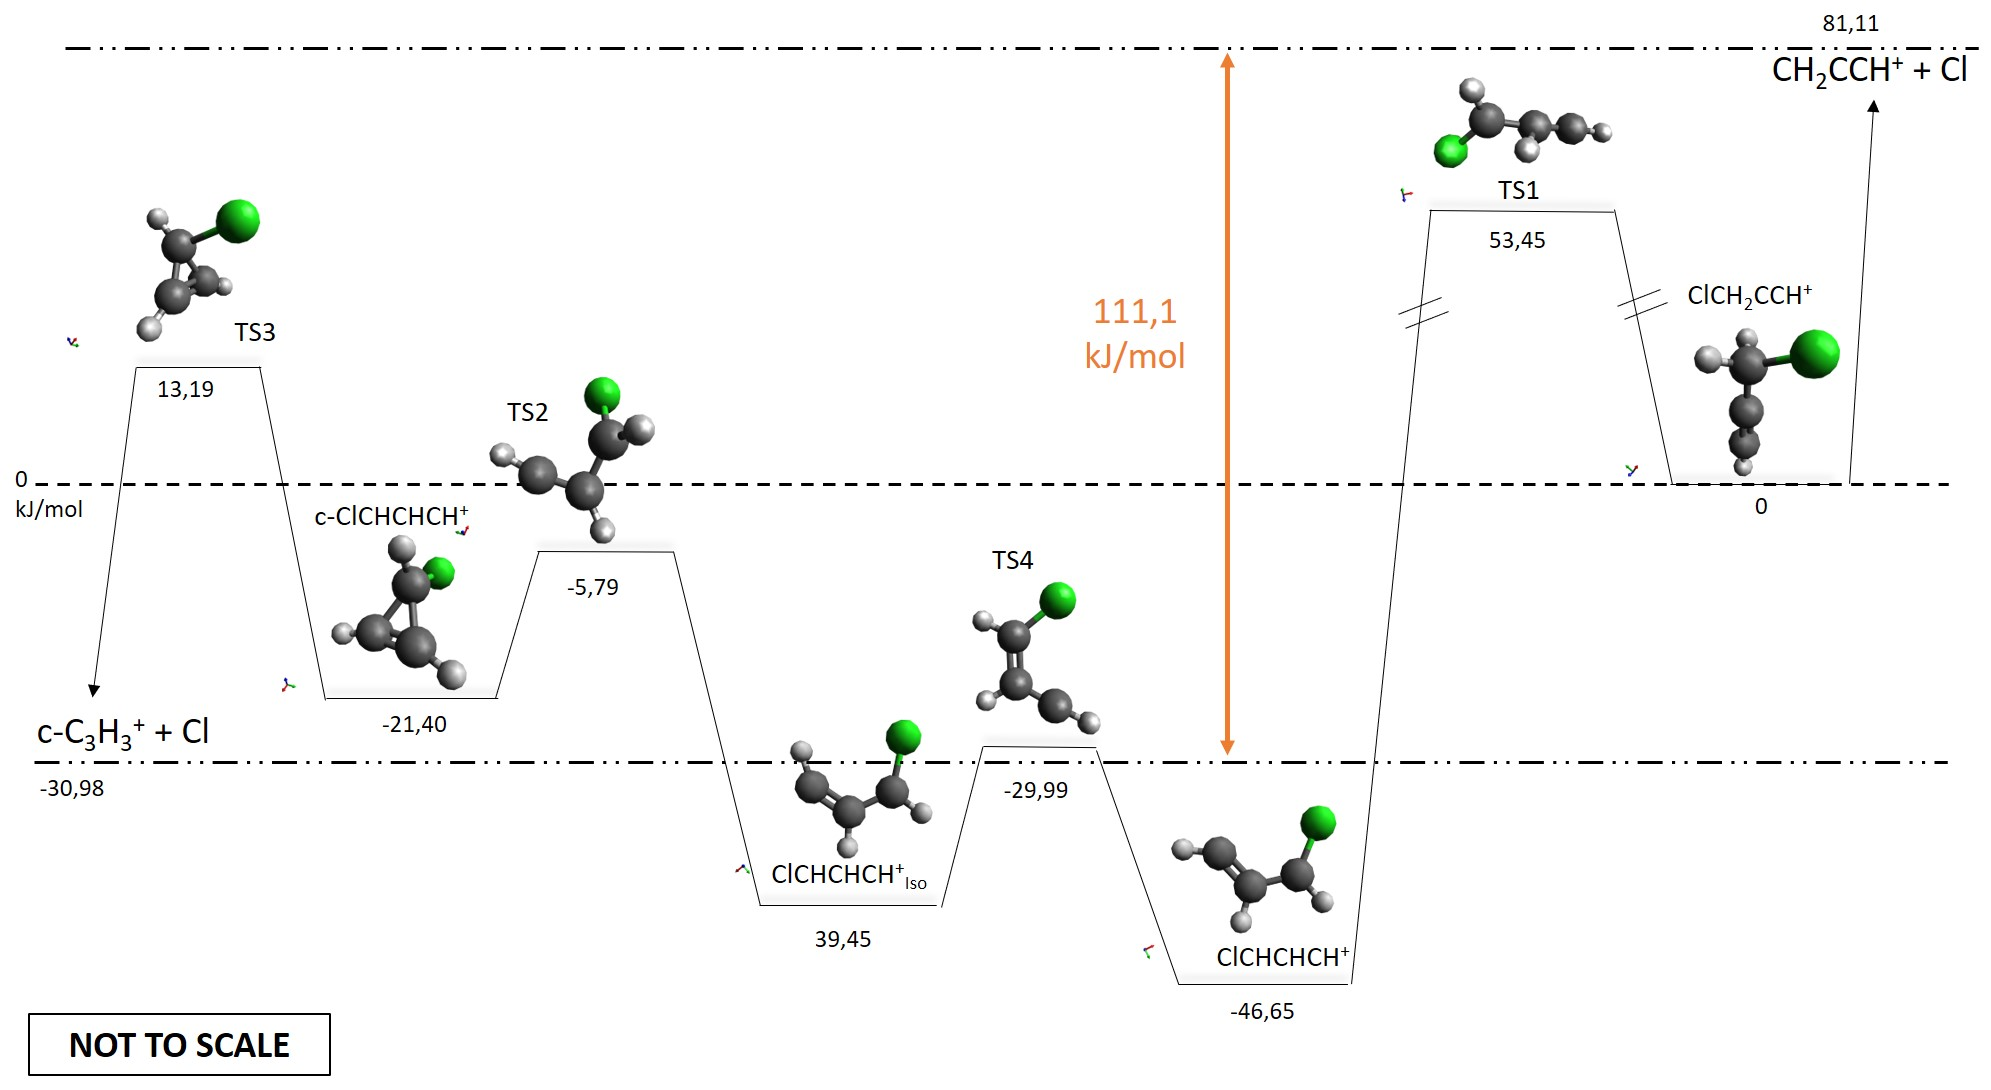
\includegraphics[width=1\textwidth]{chapters/C3H3+ and C3D3+/figures/energy_calculation.jpg}

	\caption{
        Potential energy pathway for \cyc and \lin formation from ionization of propargyl chloride (ClCH$_2$CCH). 
        The calculations are done at the CCSD(T)/cc-pVTZ level with zero-point energy corrections from MP2/cc-pVTZ level.
        The ClCH$_2$CCH$^+$ ion (propargyl chloride cation, 
        relative energy arbitrarily set  to $0\sim$kJ/mol) can undergo hydrogen migration to the linear 
        ClCHCHCH$^+$ ion (E$_ \text{rel}=-46.56\sim$kJ/mol) 
        via transition state TS1 (E$_\text{rel}=53.45\sim$kJ/mol).
        This isomer can then convert to ClCHCHCH$^+$ (iso) (E$_\text{rel}$=-30.98$\sim$kJ/mol) via TS4 (E$_\text{rel}$=-39.45$\sim$kJ/mol). 
        The latter species can subsequently cyclisise via a submerged transition state TS2 (E$_\text{rel}$=-5.79$\sim$kJ/mol) to the cyclic c-ClCHCHCH$^+$ (E$_\text{rel}$=-21.40$\sim$kJ/mol).
        This means that the highest barrier for the isomerisation of ClCH$_2$CCH$^+$ to c-ClCHCHCH$^+$ is 53.45$\sim$kJ/mol, i.e. only 0.55$\sim$eV. 
        Also the dissociation energy barrier to \cyc and Cl (E$_\text{rel}$= -29.99$\sim$kJ/mol) is only at 13.19$\sim$kJ/mol (TS3).
    }\label{fig:C3H3+:fig1}
	\label{FIG:energy_comparison}
\end{figure}
